\documentclass[crop=false, class=book]{standalone}


\usepackage{graphicx}
\usepackage[italian]{varioref}
\usepackage{copyrightbox}

\begin{document}
	\section{Comprensione Ambientale}
	\label{sec:Enviromental_Understanding}
	ARCore ha a disposizione funzione di comprensione dell’ambiente che gli consente di capire cosa circonda il dispositivo. Questa funzione è basata sulla ricerca di piani e vari punti caratteristici dell’ambiente \cite{google2022fundamentals}. \\
	\noindent
	ARCore si concentra nel trovare dei punti caratteristici posati lungo piani verticali e orizzontali così da riuscire a calcolare la posizione dei piani attraverso dei calcoli tra i sensori del dispositivo uniti al tracciamento dei punti caratteristici nell’immagine.  Inoltre, questa libreria è in grado di rilevare i bordi dei piani e utilizzare tutte queste informazioni per poter posizionare degli oggetti virtuali su di essi.\\
	\noindent
	Poiché ARCore basa la sua comprensione dell’ambiente su dei punti caratteristici, le superfici senza texture come un pavimento o un muro bianco potrebbero non essere rilevate facilmente.

	\begin{center}
		\begin{figure}[htp]
			\centering
			\copyrightbox[b]{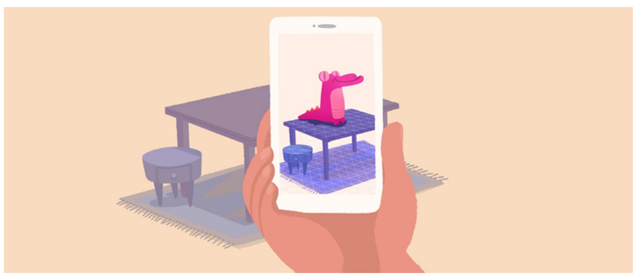
\includegraphics[width=0.9\textwidth]{./resources/images/EnvironmentalUnderstanding/env_understanding.png}}%
			{Fonte: \url{https://developers.google.com}}
			\caption{Esempio degli effetti prodotti dagli oggetti nell'ambiente.}
			\label{fig:env_und}
		\end{figure}
	\end{center}
	\noindent
	Nell'applicazione che abbiamo sviluppato questa abilità diventa fondamentale. L'oggetto posizionato viene scalato in base all'ambiente così da renderlo più realistico.
	
	\begin{center}
		\begin{figure}[htp]
		\centering
		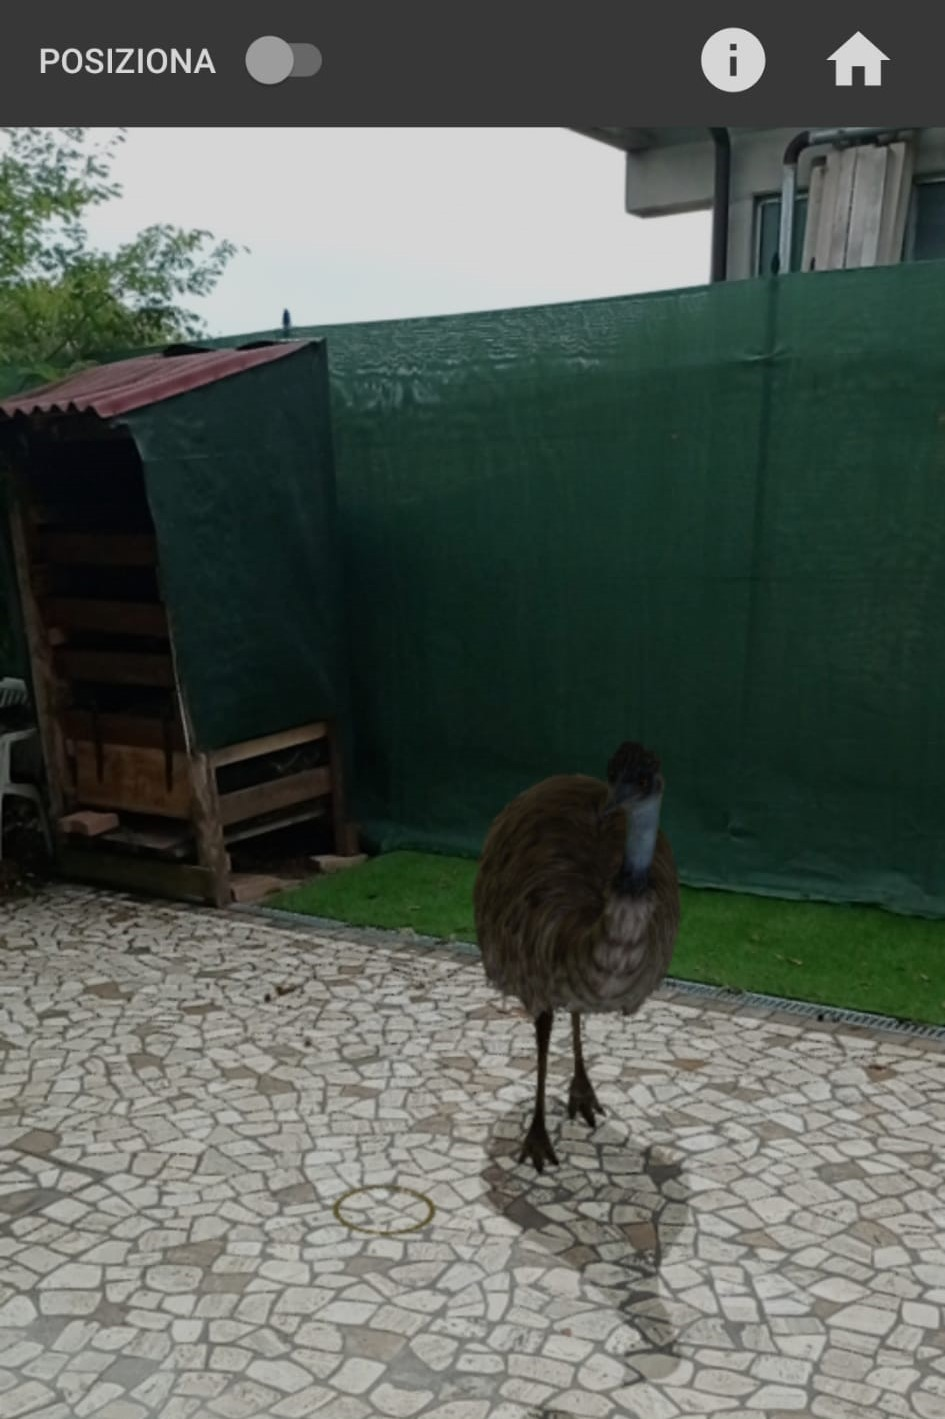
\includegraphics[width=0.5\textwidth]{./resources/images/EnvironmentalUnderstanding/env_understanding1.jpeg} 
		\caption{Esempio di immersione dell'oggetto nell'ambiente}
	\end{figure}
	
	\end{center}

\end{document}